%iffalse
\let\negmedspace\undefined
\let\negthickspace\undefined
\documentclass[journal,12pt,onecolumn]{IEEEtran}
\usepackage{cite}
\usepackage{amsmath,amssymb,amsfonts,amsthm}
\usepackage{algorithmic}
\usepackage{graphicx}
\usepackage{textcomp}
\usepackage{xcolor}
\usepackage{txfonts}
\usepackage{listings}
\usepackage{enumitem}
\usepackage{mathtools}
\usepackage{gensymb}
\usepackage{comment}
\usepackage[breaklinks=true]{hyperref}
\usepackage{tkz-euclide} 
\usepackage{listings}
\usepackage{gvv}                                        
%\def\inputGnumericTable{}                                 
\usepackage[latin1]{inputenc}     
\usepackage{xparse}
\usepackage{color}                                            
\usepackage{array}                                            
\usepackage{longtable}                                       
\usepackage{calc}                                             
\usepackage{multirow}
\usepackage{multicol}
\usepackage{hhline}                                           
\usepackage{ifthen}                                           
\usepackage{lscape}
\usepackage{tabularx}
\usepackage{array}
\usepackage{float}
\newtheorem{theorem}{Theorem}[section]
\newtheorem{problem}{Problem}
\newtheorem{proposition}{Proposition}[section]
\newtheorem{lemma}{Lemma}[section]
\newtheorem{corollary}[theorem]{Corollary}
\newtheorem{example}{Example}[section]
\newtheorem{definition}[problem]{Definition}
\newcommand{\BEQA}{\begin{eqnarray}}
\newcommand{\EEQA}{\end{eqnarray}}
\usepackage{float}
\theoremstyle{remark}
\usepackage{ circuitikz }

\title{GATE-IN-2012}
\author{EE25BTECH11002 - Achat Parth Kalpesh}
\date{}

\begin{document}

\maketitle

\section*{Questions 1-25 \brak{\text{1 mark each}}}
\begin{enumerate}
\item If $x = \sqrt{-1}$, then the value of $x^x$ is

\hfill{(GATE-IN 2012)}
\begin{enumerate}
    \begin{multicols}{2}
    \item $e^{-\pi/2}$
    \item $e^{\pi/2}$
    \item $x$
    \item $1$
    \end{multicols}
\end{enumerate}

\item With initial condition $x\brak{1} = 0.5$, the solution of the differential equation,
\begin{align*}
t\frac{dx}{dt} + x = t\text{ is}
\end{align*}

\hfill{(GATE-IN 2012)}
\begin{enumerate}
    \begin{multicols}{2}
    \item $x = t - \frac{1}{2}$
    \item $x = t^2 - \frac{1}{2}$
    \item $x = \frac{t^2}{2}$
    \item $x = \frac{t}{2}$
    \end{multicols}
\end{enumerate}

\item Two independent random variables $X$ and $Y$ are uniformly distributed in the interval $\sbrak{-1, 1}$. The probability that $\max\sbrak{X, Y}$ is less than $1/2$ is

\hfill{(GATE-IN 2012)}
\begin{enumerate}
    \begin{multicols}{4}
    \item $3/4$
    \item $9/16$
    \item $1/4$
    \item $2/3$
    \end{multicols}
\end{enumerate}

\item The unilateral Laplace transform of $f\brak{t}$ is $\frac{1}{s^2+s+1}$. The unilateral Laplace transform of $t f\brak{t}$ is

\hfill{(GATE-IN 2012)}
\begin{enumerate}
    \begin{multicols}{2}
    \item $\frac{s}{\brak{s^2+s+1}^2}$
    \item $\frac{2s+1}{\brak{s^2+s+1}^2}$
    \item $\frac{-s}{\brak{s^2+s+1}^2}$
    \item $\frac{-2s-1}{\brak{s^2+s+1}^2}$
    \end{multicols}
\end{enumerate}

\item Given
$f\brak{z} = \frac{1}{z+1} - \frac{2}{z+3}$. If C is a counterclockwise path in the z-plane such that $\abs{z+1}=1$, the value of $\frac{1}{2\pi j} \oint_C f\brak{z}dz$ is

\hfill{(GATE-IN 2012)}
\begin{enumerate}
    \begin{multicols}{4}
    \item $-2$
    \item $-1$
    \item $1$
    \item $2$
    \end{multicols}
\end{enumerate}

\item The average power delivered to an impedance $\brak{4 - j3} \ohm$ by a current $5\cos\brak{100\pi t+100}$ A is

\hfill{(GATE-IN 2012)}
\begin{enumerate}
    \begin{multicols}{4}
    \item $44.2$ W
    \item $50$ W
    \item $62.5$ W
    \item $125$ W
    \end{multicols}
\end{enumerate}

\item In the circuit shown below,\figref{fig:a1} the current through the inductor is
\begin{figure}[H]
    \centering
    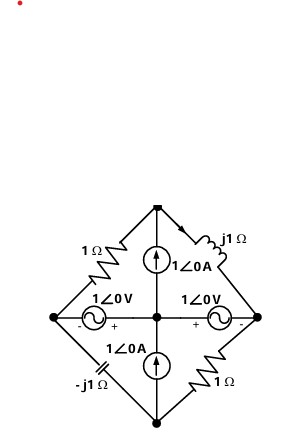
\includegraphics[width=0.6\columnwidth]{figs/a1.jpg}
    \caption*{}
    \label{fig:a1}
\end{figure}

\hfill{(GATE-IN 2012)}
\begin{enumerate}
    \begin{multicols}{2}
    \item $\frac{2}{1+j}$ A
    \item $\frac{-1}{1+j}$ A
    \item $\frac{1}{1+j}$ A
    \item $0$ A
    \end{multicols}
\end{enumerate}

\item In the following figure,\figref{fig:a2} $C_1$ and $C_2$ are ideal capacitors. $C_1$ has been charged to $12$ V before the ideal switch S is closed at $t=0$. The current $i\brak{t}$ for all $t$ is
\begin{figure}[H]
    \centering
    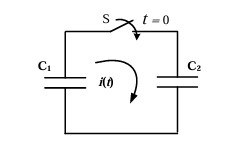
\includegraphics[width=0.5\columnwidth]{figs/a2.jpg}
    \caption*{}
    \label{fig:a2}
\end{figure}

\hfill{(GATE-IN 2012)}
\begin{enumerate}
    \begin{multicols}{2}
    \item zero
    \item a step function
    \item an exponentially decaying function
    \item an impulse function
    \end{multicols}
\end{enumerate}

\item The impedance looking into nodes 1 and 2 in the given circuit\figref{fig:a3} is
\begin{figure}[H]
    \centering
    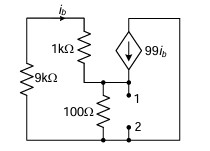
\includegraphics[width=0.4\columnwidth]{figs/a3.jpg}
    \caption*{}
    \label{fig:a3}
\end{figure}

\hfill{(GATE-IN 2012)}
\begin{enumerate}
    \begin{multicols}{2}
    \item $50 \ohm$
    \item $100 \ohm$
    \item $5$ k$\ohm$
    \item $10.1$ k$\ohm$
    \end{multicols}
\end{enumerate}

\item The i-v characteristics of the diode in the circuit given below\figref{fig:a4} are
\begin{align*} 
i = \begin{cases} \frac{v-0.7}{500} \text{A}, & v \geq 0.7 \text{ V} \\ 0 \text{ A}, & v < 0.7 \text{ V} \end{cases}
\end{align*}
\begin{figure}[H]
    \centering
    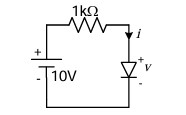
\includegraphics[width=0.4\columnwidth]{figs/a4.jpg}
    \caption*{}
    \label{fig:a4}
\end{figure}
The current in the circuit is

\hfill{(GATE-IN 2012)}
\begin{enumerate}
    \begin{multicols}{2}
    \item $10$ mA
    \item $9.3$ mA
    \item $6.67$ mA
    \item $6.2$ mA
    \end{multicols}
\end{enumerate}

\item A system with transfer function $G\brak{s} = \frac{\brak{s^2+9}\brak{s+2}}{\brak{s+1}\brak{s+3}\brak{s+4}}$ is excited by $\sin\brak{\omega t}$. The steady-state output of the system is zero at

\hfill{(GATE-IN 2012)}
\begin{enumerate}
    \begin{multicols}{2}
    \item $\omega=1$ rad/s
    \item $\omega=2$ rad/s
    \item $\omega=3$ rad/s
    \item $\omega=4$ rad/s
    \end{multicols}
\end{enumerate}

\item The output Y of a 2-bit comparator is logic 1 whenever the 2-bit input A is greater than the 2-bit input B. The number of combinations for which the output is logic 1, is

\hfill{(GATE-IN 2012)}
\begin{enumerate}
    \begin{multicols}{4}
    \item 4
    \item 6
    \item 8
    \item 10
    \end{multicols}
\end{enumerate}

\item In the sum of products function $f\brak{X, Y, Z} = \sum\brak{2, 3, 4, 5}$, the prime implicants are

\hfill{(GATE-IN 2012)}
\begin{enumerate}
    \begin{multicols}{2}
    \item $\overline{X}Y, X\overline{Y}$
    \item $\overline{X}Y, X\overline{Y}\overline{Z}, X\overline{Y}Z$
    \item $X\overline{Y}Z, \overline{X}YZ, X\overline{Y}$
    \item $\overline{X}YZ, \overline{X}Y\overline{Z}, X\overline{Y}Z, X\overline{Y}\overline{Z}$
    \end{multicols}
\end{enumerate}

\item Consider the given circuit.\figref{fig:a5}
\begin{figure}[H]
    \centering
    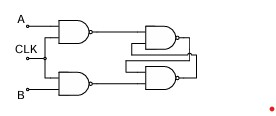
\includegraphics[width=0.6\columnwidth]{figs/a5.jpg}
    \caption*{}
    \label{fig:q14}
\end{figure}
In this circuit, the race around

\hfill{(GATE-IN 2012)}
\begin{enumerate}
    \begin{multicols}{2}
    \item does not occur
    \item occurs when CLK = 0
    \item occurs when CLK = 1 and A = B = 1
    \item occurs when CLK = 1 and A = B = 0
    \end{multicols}
\end{enumerate}

\item If $x\sbrak{n}=\brak{1/3}^{\abs{n}} - \brak{1/2}^n u\sbrak{n}$, then the region of convergence \brak{ROC} of its Z-transform in the Z-plane will be

\hfill{(GATE-IN 2012)}
\begin{enumerate}
    \begin{multicols}{2}
    \item $\frac{1}{3} < \abs{z} < 3$
    \item $\frac{1}{3} < \abs{z} < \frac{1}{2}$
    \item $\frac{1}{2} < \abs{z} < 3$
    \item $\frac{1}{3} < \abs{z}$
    \end{multicols}
\end{enumerate}

\item A capacitive motion transducer circuit is shown.\figref{fig:a6} The gap $d$ between the parallel plates of the capacitor is varied as $d\brak{t}=10^{-3}\sbrak{1+0.1\sin\brak{1000\pi t}}$ m. If the value of the capacitance is 2pF at $t=0$ ms, the output voltage $V_o$ at $t=2$ ms is
\begin{figure}[H]
    \centering
    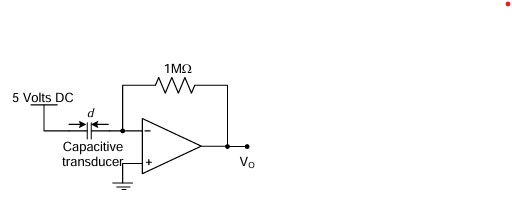
\includegraphics[width=0.5\columnwidth]{figs/a6.jpg}
    \caption*{}
    \label{fig:a6}
\end{figure}

\hfill{(GATE-IN 2012)}
\begin{enumerate}
    \begin{multicols}{2}
    \item $\frac{\pi}{2}$ mV
    \item $\pi$ mV
    \item $2\pi$ mV
    \item $4\pi$ mV
    \end{multicols}
\end{enumerate}

\item A psychrometric chart is used to determine

\hfill{(GATE-IN 2012)}
\begin{enumerate}
    \begin{multicols}{2}
    \item pH
    \item Sound velocity in glasses
    \item $CO_2$ concentration
    \item Relative humidity
    \end{multicols}
\end{enumerate}

\item A strain gauge is attached on a cantilever beam as shown.\figref{fig:a7} If the base of the cantilever vibrates according to the equation $x\brak{t} = \sin \omega_1 t + \sin \omega_2 t$, where $2 \text{ rad/s} < \omega_1, \omega_2 < 3 \text{ rad/s}$, then the output of the strain gauge is proportional to
\begin{figure}[H]
    \centering
    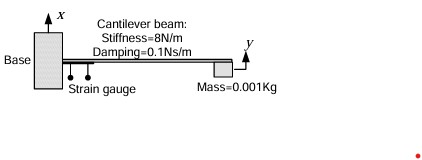
\includegraphics[width=0.7\columnwidth]{figs/a7.jpg}
    \caption*{}
    \label{fig:a7}
\end{figure}

\hfill{(GATE-IN 2012)}
\begin{enumerate}
    \begin{multicols}{2}
    \item $x$
    \item $\frac{dx}{dt}$
    \item $\frac{d^2x}{dt^2}$
    \item $\frac{d\brak{x-y}}{dt}$
    \end{multicols}
\end{enumerate}

\item The transfer function of a Zero-Order-Hold system with sampling interval T is

\hfill{(GATE-IN 2012)}
\begin{enumerate}
    \begin{multicols}{2}
    \item $\frac{1}{s}\brak{1-e^{-Ts}}$
    \item $\frac{1}{s}\brak{1-e^{-Ts}}^2$
    \item $\frac{1}{s}e^{-Ts}$
    \item $\frac{1}{s^2}e^{-Ts}$
    \end{multicols}
\end{enumerate}

\item An LED emitting at $1 \mu m $ with a spectral width of $50$ nm is used in a Michelson interferometer. To obtain a sustained interference, the maximum optical path difference between the two arms of the interferometer is

\hfill{(GATE-IN 2012)}
\begin{enumerate}
    \begin{multicols}{4}
    \item $200 \mu m$
    \item $20 \mu m$
    \item $1 \mu m$
    \item $50 nm$
    \end{multicols}
\end{enumerate}

\item Light of wavelength $630$ nm in vacuum, falling normally on a biological specimen of thickness $10 \mu m$, splits into two beams that are polarized at right angles. The refractive index of the tissue for the two polarizations are $1.32$ and $1.333$. When the two beams emerge, they are out of phase by

\hfill{(GATE-IN 2012)}
\begin{enumerate}
    \begin{multicols}{4}
    \item $0.13\degree$
    \item $74.3\degree$
    \item $90.0\degree$
    \item $128.6\degree$
    \end{multicols}
\end{enumerate}

\item The responsivity of the PIN photodiode shown\figref{fig:a8} is $0.9$ A/W. To obtain $V_{out}$ of $-1$ V for an incident optical power of $1$ mW, the value of R to be used is
\begin{figure}[H]
    \centering
    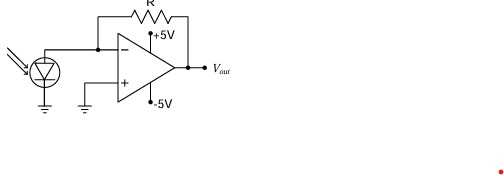
\includegraphics[width=0.5\columnwidth]{figs/a8.jpg}
    \caption*{}
    \label{fig:a8}
\end{figure}

\hfill{(GATE-IN 2012)}
\begin{enumerate}
    \begin{multicols}{4}
    \item $0.9 \ohm$
    \item $1.1 \ohm$
    \item $0.9$ k$\ohm$
    \item $1.1$ k$\ohm$
    \end{multicols}
\end{enumerate}

\item A periodic voltage waveform observed on an oscilloscope across a load is shown.\figref{fig:a9} A permanent magnet moving coil \brak{PMMC} meter connected across the same load reads
\begin{figure}[H]
    \centering
    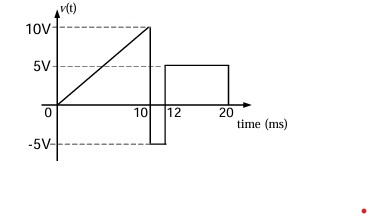
\includegraphics[width=0.6\columnwidth]{figs/a9.jpg}
    \caption*{}
    \label{fig:a9}
\end{figure}

\hfill{(GATE-IN 2012)}
\begin{enumerate}
    \begin{multicols}{4}
    \item 4 V
    \item 5 V
    \item 8 V
    \item 10 V
    \end{multicols}
\end{enumerate}

\item For the circuit shown in the figure,\figref{fig:a10} the voltage and current expressions are
\begin{align*}
v\brak{t} = E_1 \sin\brak{\omega t} + E_3 \sin\brak{3\omega t} and i\brak{t} = I_1 \sin\brak{\omega t - \phi_1} + I_3 \sin\brak{3\omega t - \phi_3} + I_5 \sin\brak{5\omega t}.
\end{align*}
The average power measured by the Wattmeter is
\begin{figure}[H]
    \centering
    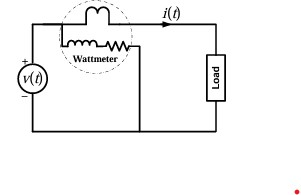
\includegraphics[width=0.4\columnwidth]{figs/a10.jpg}
    \caption*{}
    \label{fig:a10}
\end{figure}

\hfill{(GATE-IN 2012)}
\begin{enumerate}
    \begin{multicols}{2}
    \item $\frac{1}{2} E_1 I_1 \cos \phi_1$
    \item $\frac{1}{2} \sbrak{E_1 I_1 \cos \phi_1 + E_1 I_3 \cos \phi_3 + E_1 I_5}$
    \item $\frac{1}{2} \sbrak{E_1 I_1 \cos \phi_1 + E_3 I_3 \cos \phi_3}$
    \item $\frac{1}{2} \sbrak{E_1 I_1 \cos \phi_1 + E_3 I_1 \cos \phi_1}$
    \end{multicols}
\end{enumerate}

\item The bridge method commonly used for finding mutual inductance is

\hfill{(GATE-IN 2012)}
\begin{enumerate}
    \begin{multicols}{2}
    \item Heaviside Campbell bridge
    \item Schering bridge
    \item De Sauty bridge
    \item Wien bridge
    \end{multicols}
\end{enumerate}

\item A fair coin is tossed till a head appears for the first time. The probability that the number of required tosses is odd, is

\hfill{(GATE-IN 2012)}
\begin{enumerate}
    \begin{multicols}{4}
    \item $\frac{1}{3}$
    \item $\frac{1}{2}$
    \item $\frac{2}{3}$
    \item $\frac{3}{4}$
    \end{multicols}
\end{enumerate}

\item Given that
\begin{align}
A = \myvec{-5 & -3 \\ 2 & 0}\text{ and }I = \myvec{1 & 0 \\ 0 & 1},
\end{align}
the value of $A^3$ is

\hfill{(GATE-IN 2012)}
\begin{enumerate}
    \begin{multicols}{2}
    \item $15 A + 12 I$
    \item $19 A + 30 I$
    \item $17 A + 15 I$
    \item $17 A + 21 I$
    \end{multicols}
\end{enumerate}

\item The direction of vector $\mathbf{A}$ is radially outward from the origin, with
$\abs{\mathbf{A}} = kr^n$ where $r^2 = x^2+y^2+z^2$ and $k$ is a constant. The value of $n$ for which $\nabla \cdot \mathbf{A}=0$ is

\hfill{(GATE-IN 2012)}
\begin{enumerate}
    \begin{multicols}{4}
    \item $-2$
    \item $2$
    \item $1$
    \item $0$
    \end{multicols}
\end{enumerate}

\item The maximum value of $f\brak{x} = x^3 - 9x^2 + 24x + 5$ in the interval $\sbrak{1, 6}$ is

\hfill{(GATE-IN 2012)}
\begin{enumerate}
    \begin{multicols}{4}
    \item $21$
    \item $25$
    \item $41$
    \item $46$
    \end{multicols}
\end{enumerate}

\item Consider the differential equation
\begin{align*}
\frac{d^2y\brak{t}}{dt^2} + 2\frac{dy\brak{t}}{dt} + y\brak{t} = \delta\brak{t} \text{ with } y\brak{t}|_{t=0^-} = -2 \text{ and }\frac{dy}{dt}\Big|_{t=0^-} = 0.
\end{align*}
The numerical value of $\frac{dy}{dt}\Big|_{t=0^+}$ is

\hfill{(GATE-IN 2012)}
\begin{enumerate}
    \begin{multicols}{4}
    \item $-2$
    \item $-1$
    \item $0$
    \item $1$
    \end{multicols}
\end{enumerate}

\item If $V_A - V_B = 6$ V, then $V_C - V_D$ is\figref{fig:a11}
\begin{figure}[H]
    \centering
    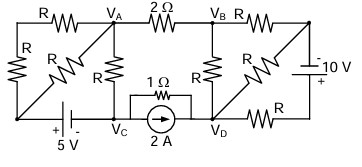
\includegraphics[width=0.5\columnwidth]{figs/a11.jpg}
    \caption*{}
    \label{fig:a11}
\end{figure}

\hfill{(GATE-IN 2012)}
\begin{enumerate}
    \begin{multicols}{4}
    \item $-5$ V
    \item $2$ V
    \item $3$ V
    \item $6$ V
    \end{multicols}
\end{enumerate}

\item Assuming both the voltage sources are in phase, the value of R for which maximum power is transferred from circuit A to circuit B is\figref{fig:a12}
\begin{figure}[H]
    \centering
    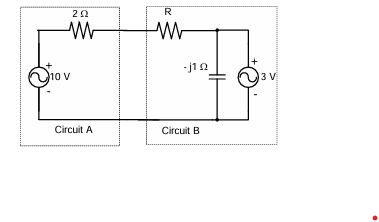
\includegraphics[width=0.7\columnwidth]{figs/a12.jpg}
    \caption*{}
    \label{fig:a12}
\end{figure}

\hfill{(GATE-IN 2012)}
\begin{enumerate}
    \begin{multicols}{4}
    \item $0.8 \ohm$
    \item $1.4 \ohm$
    \item $2 \ohm$
    \item $2.8 \ohm$
    \end{multicols}
\end{enumerate}

\item The voltage gain $A_v$ of the circuit shown below\figref{fig:a13} is
\begin{figure}[H]
    \centering
    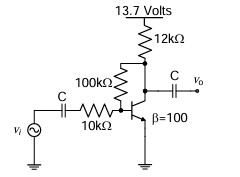
\includegraphics[width=0.6\columnwidth]{figs/a13.jpg}
    \caption*{}
    \label{fig:a13}
\end{figure}

\hfill{(GATE-IN 2012)}
\begin{enumerate}
    \begin{multicols}{4}
    \item $\abs{A_v} \approx 200$
    \item $\abs{A_v} \approx 100$
    \item $\abs{A_v} \approx 20$
    \item $\abs{A_v} \approx 10$
    \end{multicols}
\end{enumerate}

\item The state variable description of an LTI system is given by
\begin{align*}
\myvec{\dot{x_1} \\ \dot{x_2} \\ \dot{x_3}} = \myvec{0 & a_1 & 0 \\ 0 & 0 & a_2 \\ a_3 & 0 & 0} \myvec{x_1 \\ x_2 \\ x_3} + \myvec{0 \\ 0 \\ 1}u
    \end{align*}
    \begin{align*}
y = \myvec{1 & 0 & 0} \myvec{x_1 \\ x_2 \\ x_3}
    \end{align*}
where y is the output and u is the input. The system is controllable for

\hfill{(GATE-IN 2012)}
\begin{enumerate}
    \begin{multicols}{2}
    \item $a_1 \neq 0, a_2 = 0, a_3 \neq 0$
    \item $a_1 = 0, a_2 \neq 0, a_3 \neq 0$
    \item $a_1 = 0, a_2 \neq 0, a_3 = 0$
    \item $a_1 \neq 0, a_2 \neq 0, a_3 = 0$
    \end{multicols}
\end{enumerate}

\item The state transition diagram for the logic circuit shown\figref{fig:a14} is
\begin{figure}[H]
    \centering
    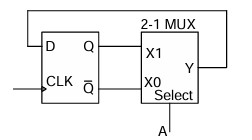
\includegraphics[width=0.5\columnwidth]{figs/a14.jpg}
    \caption*{}
    \label{fig:a14}
\end{figure}

\hfill{(GATE-IN 2012)}
 \begin{multicols}{2}
    \begin{enumerate} 
        \item  
            
       \begin{figure}[H]
    \centering
    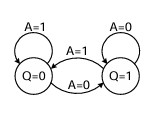
\includegraphics[width=0.5\columnwidth]{figs/a15.jpg}
    \caption{}
    \label{fig:a15}
\end{figure}
        \item  

           \begin{figure}[H]
    \centering
    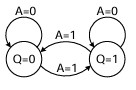
\includegraphics[width=0.5\columnwidth]{figs/a16.jpg}
    \caption{}
    \label{fig:a16}
\end{figure}
        \item  

          \begin{figure}[H]
    \centering
    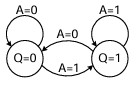
\includegraphics[width=0.5\columnwidth]{figs/a17.jpg}
    \caption{}
    \label{fig:a17}
\end{figure}
        \item 

           \begin{figure}[H]
    \centering
    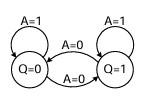
\includegraphics[width=0.5\columnwidth]{figs/a18.jpg}
    \caption{}
    \label{fig:a18}
\end{figure}
    \end{enumerate}
    \end{multicols}

\item The Fourier transform of a signal $h\brak{t}$ is $H\brak{j\omega} = j\cos\brak{2\omega} - \sin\brak{2\omega}/\omega$. The value of $h\brak{0}$ is

\hfill{(GATE-IN 2012)}
\begin{enumerate}
    \begin{multicols}{4}
    \item $1/4$
    \item $1/2$
    \item $1$
    \item $2$
    \end{multicols}
\end{enumerate}

\item Let $y\sbrak{n}$ denote the convolution of $h\sbrak{n}$ and $g\sbrak{n}$, where $h\sbrak{n}=\brak{1/2}^n u\sbrak{n}$ and $g\sbrak{n}$ is a causal sequence. If $y\sbrak{0}=1$ and $y\sbrak{1}=1/2$, then $g\sbrak{1}$ equals

\hfill{(GATE-IN 2012)}
\begin{enumerate}
    \begin{multicols}{4}
    \item $0$
    \item $1/2$
    \item $1$
    \item $3/2$
    \end{multicols}
\end{enumerate}

\item The feedback system shown below\figref{fig:a19} oscillates at $2$ rad/s when
\begin{figure}[H]
    \centering
    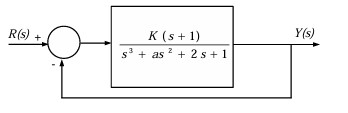
\includegraphics[width=0.8\columnwidth]{figs/a19.jpg}
    \caption*{}
    \label{fig:a19}
\end{figure}

\hfill{(GATE-IN 2012)}
\begin{enumerate}
    \begin{multicols}{2}
    \item $K = 2$ and $a = 0.75$
    \item $K = 3$ and $a = 0.75$
    \item $K = 4$ and $a = 0.5$
    \item $K = 2$ and $a = 0.5$
    \end{multicols}
\end{enumerate}

\item The circuit shown is a\figref{fig:a20}
\begin{figure}[H]
    \centering
    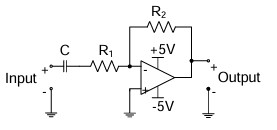
\includegraphics[width=0.6\columnwidth]{figs/a20.jpg}
    \caption*{}
    \label{fig:a20}
\end{figure}

\hfill{(GATE-IN 2012)}
\begin{enumerate}
    \item low pass filter with $f_{3dB} = \frac{1}{\brak{R_1+R_2}C}$ rad/s
    \item high pass filter with $f_{3dB} = \frac{1}{R_1 C}$ rad/s
    \item low pass filter with $f_{3dB} = \frac{1}{R_1 C}$ rad/s
    \item high pass filter with $f_{3dB} = \frac{1}{\brak{R_1+R_2}C}$ rad/s
\end{enumerate}

\item The input $x\brak{t}$ and output $y\brak{t}$ of a system are related as $y\brak{t} = \int_{-\infty}^t x\brak{\tau}\cos\brak{3\tau} d\tau$. The system is

\hfill{(GATE-IN 2012)}
\begin{enumerate}
    \begin{multicols}{2}
    \item time-invariant and stable
    \item stable and not time-invariant
    \item time-invariant and not stable
    \item not time-invariant and not stable
    \end{multicols}
\end{enumerate}

\item A double convex lens is used to couple a laser beam of diameter $5$ mm into an optical fiber with a numerical aperture of $0.5$. The minimum focal length of the lens that should be used in order to focus the entire beam into the fiber is

\hfill{(GATE-IN 2012)}
\begin{enumerate}
    \begin{multicols}{4}
    \item $1.44$ mm
    \item $2.50$ mm
    \item $4.33$ mm
    \item $5.00$ mm
    \end{multicols}
\end{enumerate}

\item An analog voltmeter uses external multiplier settings. With a multiplier setting of $20$ k$\ohm$, it reads $440$ V and with a multiplier setting of $80$ k$\ohm$, it reads $352$ V. For a multiplier setting of $40$ k$\ohm$, the voltmeter reads

\hfill{(GATE-IN 2012)}
\begin{enumerate}
    \begin{multicols}{4}
    \item $371$ V
    \item $383$ V
    \item $394$ V
    \item $406$ V
    \end{multicols}
\end{enumerate}

\item The open loop transfer function of a unity negative feedback control system is given by $G\brak{s} = \frac{150}{s\brak{s+9}\brak{s+25}}$. The gain margin of the system is

\hfill{(GATE-IN 2012)}
\begin{enumerate}
    \begin{multicols}{4}
    \item $10.8$ dB
    \item $22.3$ dB
    \item $34.1$ dB
    \item $45.6$ dB
    \end{multicols}
\end{enumerate}

\item A dynamometer arm makes contact with the piezoelectric load cell as shown.\figref{fig:a21} The g-constant of the piezoelectric material is $50 \times 10^{-3}$ Vm/N and the surface area of the load cell is $4$ $cm^2$. If a torque $\tau = 20$ Nm is applied to the dynamometer, the output voltage $V_O$ of the load cell is
\begin{figure}[H]
    \centering
    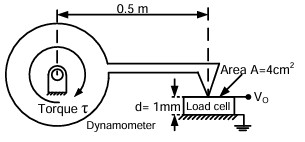
\includegraphics[width=0.8\columnwidth]{figs/a21.jpg}
    \caption*{}
    \label{fig:a21}
\end{figure}

\hfill{(GATE-IN 2012)}
\begin{enumerate}
    \begin{multicols}{4}
    \item $4$ V
    \item $5$ V
    \item $10$ V
    \item $16$ V
    \end{multicols}
\end{enumerate}

\item Water \brak{density: 1000 kgm ^{-3}} stored in a cylindrical drum of diameter 1 m is emptied through a horizontal pipe of diameter 0.05 m. A pitot-static tube is placed inside the pipe facing the flow. At the time when the difference between the stagnation and static pressures measured by the pitot-static tube is 10 kPa, the rate of reduction in water level in the drum is,

\hfill{(GATE-IN 2012)}
\begin{enumerate}
    \begin{multicols}{4}
    \item $\frac{1}{200\sqrt{5}}$ ms$^{-1}$
    \item $\frac{1}{75\sqrt{10}}$ ms$^{-1}$
    \item $\frac{1}{50\sqrt{10}}$ ms$^{-1}$
    \item $\frac{1}{40\sqrt{5}}$ ms$^{-1}$
    \end{multicols}
\end{enumerate}

\item A U-tube manometer of tube diameter $D$ is filled with a liquid of zero viscosity. If the volume of the liquid filled is $V$, the natural frequency of oscillations in the liquid level about its mean position, due to small perturbations, is

\hfill{(GATE-IN 2012)}
\begin{enumerate}
    \begin{multicols}{4}
    \item $\frac{D}{2\sqrt{2\pi}} \sqrt{\frac{g}{V}}$
    \item $\frac{2\sqrt{2}}{\sqrt{\pi}} \frac{\sqrt{gV}}{D^2}$
    \item $\frac{1}{2\sqrt{\pi}} \frac{\sqrt{gD}}{V^{1/3}}$
    \item $\frac{1}{\sqrt{\pi}} \sqrt{\frac{g}{D}}$
    \end{multicols}
\end{enumerate}

\item The open loop transfer function of a unity gain negative feedback control system is given by $G\brak{s} = \frac{s^2+4s+8}{s\brak{s+2}\brak{s+8}}$. The angle $\theta$, at which the root locus approaches the zeros of the system, satisfies

\hfill{(GATE-IN 2012)}
\begin{enumerate}
    \begin{multicols}{2}
    \item $\abs{\theta} = \pi - \tan^{-1}\brak{\frac{1}{4}}$
    \item $\abs{\theta} = \frac{3\pi}{4} - \tan^{-1}\brak{\frac{1}{3}}$
    \item $\abs{\theta} = \frac{\pi}{2} - \tan^{-1}\brak{\frac{1}{4}}$
    \item $\abs{\theta} = \frac{\pi}{4} - \tan^{-1}\brak{\frac{1}{3}}$
    \end{multicols}
\end{enumerate}

\textbf{Common Data for Questions 48 and 49:}

With 10 V dc connected at port A in the linear nonreciprocal two-port network shown below,\figref{fig:a22} the following were observed:
\begin{enumerate}
\item $1 \ohm$ connected at port B draws a current of $3$ A
\item $2.5 \ohm$ connected at port B draws a current of $2$ A
\end{enumerate}
\begin{figure}[H]
    \centering
    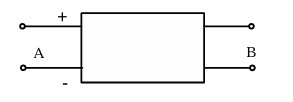
\includegraphics[width=0.6\columnwidth]{figs/a22.jpg}
    \caption*{}
    \label{fig:a22}
\end{figure}

\item With 10 V dc connected at port A, the current drawn by $7 \ohm$ connected at port B is

\hfill{(GATE-IN 2012)}
\begin{enumerate}
    \begin{multicols}{4}
    \item 3/7 A
    \item 5/7 A
    \item 1 A
    \item 9/7 A
    \end{multicols}
\end{enumerate}

\item For the same network, with 6 V dc connected at port A, $1 \ohm$ connected at port B draws 7/3 A. If 8 V dc is connected to port A, the open circuit voltage at port B is

\hfill{(GATE-IN 2012)}
\begin{enumerate}
    \begin{multicols}{4}
    \item 6 V
    \item 7 V
    \item 8 V
    \item 9 V
    \end{multicols}
\end{enumerate}

\textbf{Common Data for Questions 50 and 51:}

The deflection profile $y\brak{x}$ of a cantilever beam due to application of a point force $F$ \brak{in\ Newton}, as a function of distance $x$ from its base, is given by $y\brak{x} = 0.001F x^2 \brak{1 - \frac{x}{3}}$ m. The angular deformation $\theta$ at the end of the cantilever is measured by reflecting a laser beam off a mirror M as shown in the figure.\figref{fig:a23}

\begin{figure}[H]
    \centering
    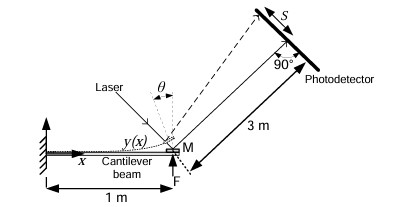
\includegraphics[width=0.5\columnwidth]{figs/a23.jpg}
    \caption*{}
    \label{fig:a23}
\end{figure}

\item The translation S of the spot of laser light on the photodetector when a force of $F=1$ N is applied to the cantilever is

\hfill{(GATE-IN 2012)}
\begin{enumerate}
    \begin{multicols}{4}
    \item 1 mm
    \item 3 mm
    \item 6 mm
    \item 12 mm
    \end{multicols}
\end{enumerate}

\item If linear variable differential transformers \brak{LVDTs} are mounted at $x=\frac{1}{2}$ m and $x=\frac{1}{4}$ m on the cantilever to measure the effect of time varying forces, the ratio of their outputs is

\hfill{(GATE-IN 2012)}
\begin{enumerate}
    \begin{multicols}{4}
    \item 12/7
    \item 40/11
    \item 176/23
    \item 112/15
    \end{multicols}
\end{enumerate}

\textbf{Statement for Linked Answer Questions 52 and 53:}

The transfer function of a compensator is given as $G_c\brak{s} = \frac{s+a}{s+b}$

\item $G_c\brak{s}$ is a lead compensator if

\hfill{(GATE-IN 2012)}
\begin{enumerate}
    \begin{multicols}{2}
    \item $a=1, b=2$
    \item $a=3, b=2$
    \item $a=-3, b=-1$
    \item $a=3, b=1$
    \end{multicols}
\end{enumerate}

\item The phase of the above lead compensator is maximum at

\hfill{(GATE-IN 2012)}
\begin{enumerate}
    \begin{multicols}{4}
    \item $\sqrt{2}$ rad/s
    \item $\sqrt{3}$ rad/s
    \item $\sqrt{6}$ rad/s
    \item $1/\sqrt{3}$ rad/s
    \end{multicols}
\end{enumerate}

\textbf{Statement for Linked Answer Questions 54 and 55:}

In the circuit shown,\figref{fig:a24} the three voltmeter readings are $V_1 = 220$ V, $V_2 = 122$ V, $V_3 = 136$ V.

\begin{figure}[H]
    \centering
    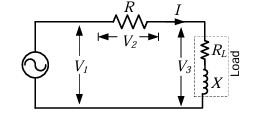
\includegraphics[width=0.4\columnwidth]{figs/a24.jpg}
    \caption*{}
    \label{fig:a24}
\end{figure}

\item The power factor of the load is

\hfill{(GATE-IN 2012)}
\begin{enumerate}
    \begin{multicols}{4}
    \item 0.45
    \item 0.50
    \item 0.55
    \item 0.60
    \end{multicols}
\end{enumerate}

\item If $R_L = 5 \ohm$, the approximate power consumption in the load is

\hfill{(GATE-IN 2012)}
\begin{enumerate}
    \begin{multicols}{4}
    \item 700 W
    \item 750 W
    \item 800 W
    \item 850 W
    \end{multicols}
\end{enumerate}

\item Choose the most appropriate alternative from the options given below to complete the following sentence:
If the tired soldier wanted to lie down, he \rule{2cm}{0.4pt} the mattress out on the balcony.

\hfill{(GATE-IN 2012)}
\begin{enumerate}
    \item should take
    \item shall take
    \item should have taken
    \item will have taken
\end{enumerate}

\item If $\brak{1.001}^{1259} = 3.52$ and $\brak{1.001}^{2062} = 7.85$, then $\brak{1.001}^{3321} =$

\hfill{(GATE-IN 2012)}
\begin{enumerate}
    \begin{multicols}{4}
    \item 2.23
    \item 4.33
    \item 11.37
    \item 27.64
    \end{multicols}
\end{enumerate}

\item One of the parts \brak{A, B, C, D} in the sentence given below contains an ERROR. Which one of the following is INCORRECT?
I requested that he should be given the driving test today instead of tomorrow.

\hfill{(GATE-IN 2012)}
\begin{enumerate}
    \item requested that
    \item should be given
    \item the driving test
    \item instead of tomorrow
\end{enumerate}

\item Which one of the following options is the closest in meaning to the word given below?
Latitude

\hfill{(GATE-IN 2012)}
\begin{enumerate}
    \begin{multicols}{4}
    \item Eligibility
    \item Freedom
    \item Coercion
    \item Meticulousness
    \end{multicols}
\end{enumerate}

\item Choose the most appropriate word from the options given below to complete the following sentence:
Given the seriousness of the situation that he had to face, his \rule{2cm}{0.4pt} was impressive.

\hfill{(GATE-IN 2012)}
\begin{enumerate}
    \begin{multicols}{4}
    \item beggary
    \item nomenclature
    \item jealousy
    \item nonchalance
    \end{multicols}
\end{enumerate}

\textbf{Q. 61 - Q. 65 carry two marks each. }


\item Raju has 14 currency notes in his pocket consisting of only Rs. 20 notes and Rs. 10 notes. The total money value of the notes is Rs. 230. The number of Rs. 10 notes that Raju has is

\hfill{(GATE-IN 2012)}
\begin{enumerate}
    \begin{multicols}{4}
    \item 5
    \item 6
    \item 9
    \item 10
    \end{multicols}
\end{enumerate}

\item One of the legacies of the Roman legions was discipline. In the legions, military law prevailed and discipline was brutal. Discipline on the battlefield kept units obedient, intact and fighting, even when the odds and conditions were against them.

Which one of the following statements best sums up the meaning of the above passage?

\hfill{(GATE-IN 2012)}
\begin{enumerate}
    \item Thorough regimentation was the main reason for the efficiency of the Roman legions even in adverse circumstances.
    \item The legions were treated inhumanly as if the men were animals.
    \item Discipline was the armies' inheritance from their seniors.
    \item The harsh discipline to which the legions were subjected to led to the odds and conditions being against them.
\end{enumerate}

\item A and B are friends. They decide to meet between 1 PM and 2 PM on a given day. There is a condition that whoever arrives first will not wait for the other for more than 15 minutes. The probability that they will meet on that day is

\hfill{(GATE-IN 2012)}
\begin{enumerate}
    \begin{multicols}{4}
    \item 1/4
    \item 1/16
    \item 7/16
    \item 9/16
    \end{multicols}
\end{enumerate}

\item The data given in the following table summarizes the monthly budget of an average household.

\begin{table}[h]
\centering
\begin{tabular}{|l|c|}
\hline
\textbf{Category} & \textbf{Amount \brak{Rs.}} \\ \hline
Food & 4000 \\ \hline
Clothing & 1200 \\ \hline
Rent & 2000 \\ \hline
Savings & 1500 \\ \hline
Other expenses & 1800 \\ \hline
\end{tabular}
\caption*{}
\label{tab:2}
\end{table}

The approximate percentage of the monthly budget NOT spent on savings is

\hfill{(GATE-IN 2012)}
\begin{enumerate}
    \begin{multicols}{4}
    \item 10\%
    \item 14\%
    \item 81\%
    \item 86\%
    \end{multicols}
\end{enumerate}

\item There are eight bags of rice looking alike, seven of which have equal weight and one is slightly heavier. The weighing balance is of unlimited capacity. Using this balance, the minimum number of weighings required to identify the heavier bag is

\hfill{(GATE-IN 2012)}
\begin{enumerate}
    \begin{multicols}{4}
    \item 2
    \item 3
    \item 4
    \item 8
    \end{multicols}
\end{enumerate}

\section*{End of the question Paper.}

\end{enumerate}
\end{document}